\documentclass[border=3pt,tikz]{standalone}
\usepackage{amsmath}
\usetikzlibrary{calc}
\usetikzlibrary{arrows.meta} % for arrow size
\begin{document}
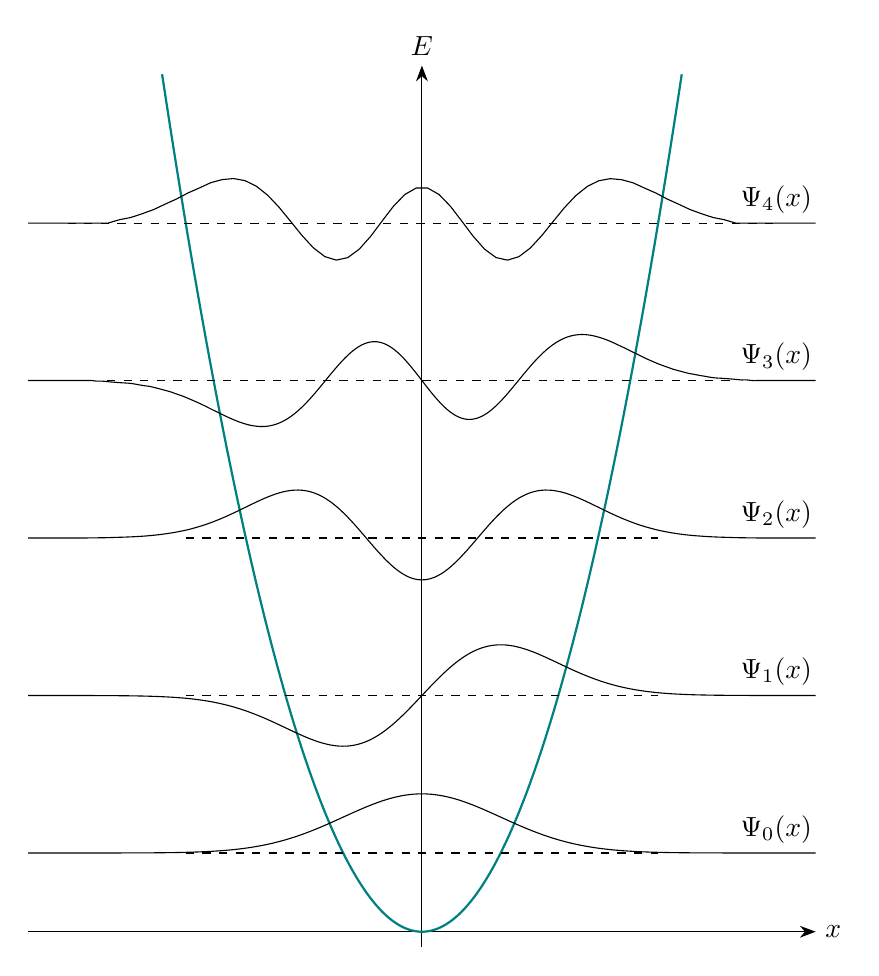
\begin{tikzpicture}[scale=1.0]
    \usetikzlibrary {arrows.meta}
    \usetikzlibrary {calc}
    
    \draw[, -{Stealth[length=2mm]}] (-5, 0) -- (5, 0) node [right] {$x$} ;
    \draw[, -{Stealth[length=2mm]}] (0, -0.2) -- (0, 11) node [above] {$E$};
    
    
    \draw[teal, thick] plot[variable=\t, domain=-3.3:3.3, samples=100, smooth,thick] ({\t}, {\t*\t});
    
    
    \draw[] plot[variable=\t, domain=-5:5, samples=100, smooth,thick] ({\t}, {0.751*exp(-(\t*\t)/2) + 1.0});
    \draw[dashed] (-3, 1) -- (3, 1);
    \node[above] at (4.5, 1) {$\Psi_0(x)$};
    
    \draw[] plot[variable=\t, domain=-5:5, samples=100, smooth,thick] ({\t}, {0.531*exp(-(\t*\t)/2) *(2*\t) + 3.0});
    \draw[dashed] (-3, 3) -- (3, 3);
    \node[above] at (4.5, 3) {$\Psi_1(x)$};
    
    \draw[] plot[variable=\t, domain=-5:5, samples=100, smooth,thick] ({\t}, {0.266 * exp(-(\t*\t)/2) *(-2*(1-2*\t*\t)) + 5.0});
    \draw[dashed] (-3, 5) -- (3, 5);
    \node[above] at (4.5, 5) {$\Psi_2(x)$};
    
    \draw[] plot[variable=\t, domain=-5:5, samples=150, smooth,thick] ({\t}, {0.108 * exp(-(\t*\t)/2) *(-12*(\t-0.666*\t*\t*\t)) + 7.0});
    \draw[dashed] (-4, 7) -- (4, 7);
    \node[above] at (4.5, 7) {$\Psi_3(x)$};
    
    \draw[] plot[variable=\t, domain=-5:5, samples=70,thick] ({\t}, {0.038 * exp(-((\t)^2)/2) *(12*(1-4*((\t)^2)+4/3*((\t)^4))) + 9.0});
    \draw[dashed] (-4.5, 9) -- (4.5, 9);
    \node[above] at (4.5, 9) {$\Psi_4(x)$};
    
    \end{tikzpicture}
\end{document}